\documentclass[tikz]{standalone}


\usetikzlibrary{shapes, shapes.geometric, shapes.misc, shapes.arrows}
%\usetikzlibrary{3d, perspective}
\usetikzlibrary{arrows, arrows.meta}
\usetikzlibrary{angles, math, calc, matrix}
\usetikzlibrary{positioning}
\usetikzlibrary{decorations.pathreplacing, decorations.markings, decorations.text, calligraphy}

\begin{document}

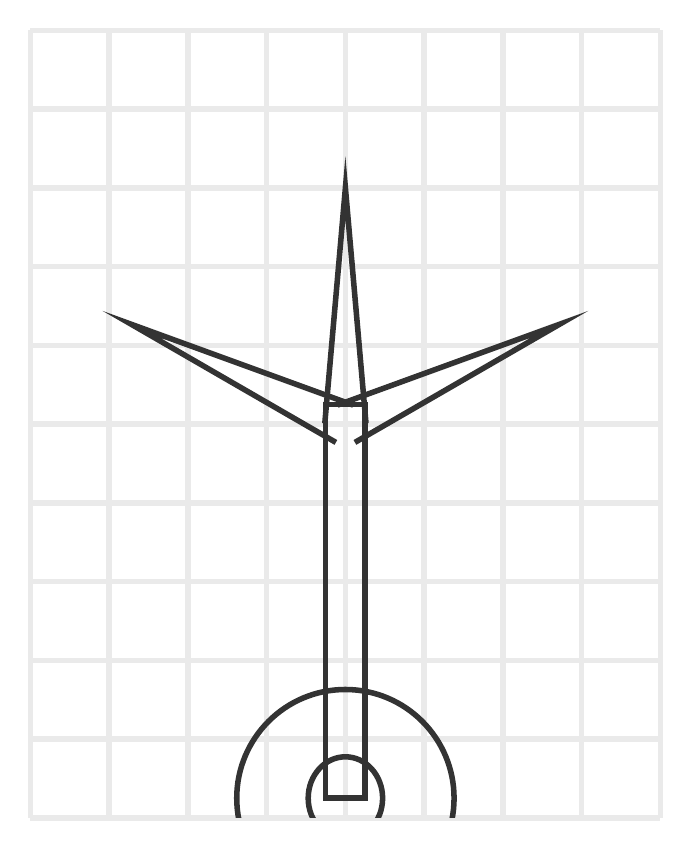
\begin{tikzpicture}[black!80, line width = 2pt]

    \def\Ybound{10}
    \def\Xbound{4}

    \draw[opacity = 0.1] (-\Xbound,-0) grid (\Xbound,\Ybound);
    \clip[use as bounding box] (-\Xbound,-0) rectangle (\Xbound,\Ybound);

    \def\nuclea{0.35}
    \def\radius{2.3}
    \def\angle{65}
    \def\angledos{5}

    \coordinate (O) at (0,0.25);

    \begin{scope}[scale = 0.60, transform shape]
        \draw (O) circle (\radius);
        \draw[rounded corners, rotate = 90]  
                (O) ellipse [x radius= 2.5*\nuclea , y radius= 2.25*\nuclea ];
    \end{scope}
    
    \path (0,0) -- (0,5) coordinate (Junc);
    \path foreach \SIGN/\PEAK in {-/I,\angle-/II,+/III} 
        {(Junc) -- ([turn]\SIGN \angle:3) coordinate (S\PEAK)};

    \foreach \CENTER/\ANG in {SI/-90-\angle, SII/-90, SIII/+\angle-90}{
        \begin{scope}[shift = (\CENTER), rotate = \ANG]
            \draw[miter limit = 25] 
                {(-\angledos:3) -- (\CENTER) -- (+\angledos:3)};
        \end{scope}}

    
    \draw (O)+(0:0.25) rectangle +(-0.25,5);


\end{tikzpicture}

\end{document}